\documentclass[11pt,a4paper]{article}

\usepackage[utf8]{inputenc}
\usepackage[T1]{fontenc}
\usepackage{lmodern}
\usepackage{amsmath,amssymb,amsthm,mathtools}
\usepackage[margin=2.5cm]{geometry}
\usepackage{hyperref}
\usepackage{cleveref}
\usepackage{enumitem}
\usepackage{booktabs}
\usepackage{xcolor}
\usepackage{fancyhdr}
\usepackage{longtable}
\usepackage{graphicx}

\newcommand{\dd}{\mathrm{d}}
\newcommand{\PiTT}{\Pi_{\mathrm{TT}}}
\newcommand{\PiS}{\Pi_{\mathrm{s}}}
\newcommand{\Fhat}{\hat{F}}
\newcommand{\order}{\mathcal{O}}
\newcommand{\MPl}{M_{\mathrm{Pl}}}
\newcommand{\Imag}{\mathrm{Im}}
\newcommand{\Real}{\mathrm{Re}}
\newcommand{\Lam}{\Lambda}

\newtheorem{theorem}{Theorem}[section]
\newtheorem{proposition}[theorem]{Proposition}
\newtheorem{corollary}[theorem]{Corollary}
\newtheorem{remark}[theorem]{Remark}

\pagestyle{fancy}
\fancyhf{}
\fancyhead[L]{\small\textsc{SCT Theory --- MR-3}}
\fancyhead[R]{\small\thepage}
\renewcommand{\headrulewidth}{0.4pt}

\hypersetup{
  colorlinks=true,
  linkcolor=blue!60!black,
  citecolor=green!40!black,
  urlcolor=blue!60!black,
  pdftitle={MR-3: Causality Analysis of the SCT Nonlocal Graviton Propagator},
  pdfauthor={David Alfyorov},
}

\title{%
  \textbf{MR-3: Causality Analysis}\\[4pt]
  \textbf{of the SCT Nonlocal Graviton Propagator}\\[6pt]
  \large Retarded Green's Function, Kramers--Kronig Relations,\\
  Initial Value Problem, and Macrocausality
}
\author{David Alfyorov}
\date{March 2026}

\begin{document}
\maketitle

\begin{center}
and workflow support.}
\end{center}

\tableofcontents
\newpage

% ==========================================================================
\section{Introduction}
\label{sec:intro}
% ==========================================================================

This document presents the causality analysis of the Spectral Causal Theory
(SCT) nonlocal graviton propagator, addressing all five subtasks of the MR-3
milestone. The central object is the spin-2 transverse-traceless propagator
denominator:
\begin{equation}\label{eq:PiTT}
  \PiTT(z) = 1 + \frac{13}{60}\,z\,\Fhat_1(z),
  \qquad z = \frac{k^2}{\Lam^2},
\end{equation}
where $\Fhat_1(z) = F_1(z)/F_1(0)$ is the normalized form factor built from
the master function
\begin{equation}\label{eq:phi}
  \varphi(z) = e^{-z/4}\sqrt{\frac{\pi}{z}}\,\mathrm{erfi}\!\left(\frac{\sqrt{z}}{2}\right),
\end{equation}
an entire function of order~1 and type~$1/4$ with real Taylor coefficients
$a_n = (-1)^n\,n!/(2n+1)!$\,.

\medskip\noindent
\textbf{Key physics.} The SCT propagator has an infinite tower of ghost poles
(zeros of $\PiTT(z)$), including one real Lorentzian pole at $z_L \approx -1.2807$
and one real Euclidean pole at $z_0 \approx 2.4148$, plus an infinite sequence
of complex Lee--Wick pairs. The physical S-matrix uses the fakeon (principal
value) prescription at ghost poles, which trades strict microcausality for
unitarity. This tradeoff is the central theme of the analysis.

\medskip\noindent
\textbf{Classification.} Within the taxonomy of higher-derivative/nonlocal
gravity theories, the SCT belongs to a distinct class:
\begin{itemize}[nosep]
  \item \textbf{Class~I} (ghost-free): $\exp(H(\Box))$ theories
    (Tomboulis~\cite{Tomboulis1997}, Modesto~\cite{GiaccariModesto2018}).
    No ghost poles, full microcausality.
  \item \textbf{Class~II} (polynomial): Stelle gravity~\cite{Stelle1977}.
    One ghost pole, microcausality violated at $1/m_{\text{Stelle}}$.
  \item \textbf{Class~III} (entire with zeros): SCT. Infinite ghost tower,
    microcausality violated at $\sim 1/\Lam$.
    Closest comparison: Anselmi's fakeon quantum gravity~\cite{AnselmiPiva2018}.
\end{itemize}

\medskip\noindent
\textbf{Overall verdict: CONDITIONAL.} Macrocausality is preserved at distances
$r \gg 1/\Lam$. The front velocity equals $c$. Kramers--Kronig relations are
trivially satisfied at tree level. The initial value problem is well-posed
(perturbative and classicized). Microcausality is violated at scale $\sim 1/\Lam$,
which is an inherent and well-understood feature of the fakeon prescription.

% ==========================================================================
\section{Sub-task (a): Retarded Green's Function}
\label{sec:retarded}
% ==========================================================================

\subsection{Pole decomposition}

The Hadamard function (GZ result) decomposes the propagator as:
\begin{equation}\label{eq:pole-decomp}
  H(z) = \frac{1}{z\,\PiTT(z)}
  = g_A + \frac{1}{z} + \sum_n R_n\left[\frac{1}{z - z_n} + \frac{1}{z_n}\right],
\end{equation}
where $g_A = -c_2 = -13/60$ is the entire part and the sum runs over all zeros
$z_n$ of $\PiTT(z)$ with residues $R_n = 1/(z_n\,\PiTT'(z_n))$.

Each pole contributes to the position-space Green's function:
\begin{itemize}[nosep]
  \item \textbf{Graviton} ($z=0$): massless retarded propagator, supported on
    the forward light cone $\{t > 0,\; t^2 = r^2\}$.
  \item \textbf{Ghost poles} ($z_n \neq 0$): massive retarded propagator of mass
    $m_n = \Lam\sqrt{|z_n|}$, supported inside the forward light cone
    $\{t > 0,\; t^2 > r^2\}$.
\end{itemize}

\subsection{Retarded vs.\ fakeon propagator}

The retarded propagator $G_{\mathrm{ret}}(t,r;m)$ vanishes for $t < 0$ and for
spacelike separations $t^2 < r^2$. For a massive scalar inside the forward
light cone ($t > r > 0$):
\begin{equation}\label{eq:Gret-massive}
  G_{\mathrm{ret}}(t,r;m) = \frac{m\,J_1(m\tau)}{4\pi\tau},
  \qquad \tau = \sqrt{t^2 - r^2}\,.
\end{equation}

The fakeon (PV) propagator is the average of retarded and advanced:
\begin{equation}\label{eq:GFK}
  G_{\mathrm{FK}}(t,r;m) = \tfrac{1}{2}\left[G_{\mathrm{ret}}(t,r;m)
  + G_{\mathrm{ret}}(-t,r;m)\right].
\end{equation}
This is nonzero for $t < 0$ (past timelike), violating microcausality.
Crucially, $G_{\mathrm{FK}}$ still vanishes for spacelike separations,
so no superluminal signal propagation occurs.

\subsection{Numerical verification}

\begin{table}[htbp]
\centering
\caption{Support properties of $G_{\mathrm{ret}}$ and $G_{\mathrm{FK}}$ at
selected spacetime points ($\Lam = 1$).}
\label{tab:propagator-support}
\begin{tabular}{@{}lrrcccc@{}}
\toprule
Label & $t$ & $r$ & Region & $G_{\mathrm{ret}}$ & $G_{\mathrm{FK}}$ & Expected \\
\midrule
Future timelike & 2.0 & 0.5 & Timelike & $-2.45\times10^{-2}$ & $-1.23\times10^{-2}$ & $\neq 0$ \\
Lightlike       & 1.0 & 1.0 & Light cone & 0 & 0 & 0 \\
Spacelike       & 0.5 & 2.0 & Spacelike & 0 & 0 & 0 \\
Equal time      & 0.0 & 1.0 & Spacelike & 0 & 0 & 0 \\
Past timelike   & $-1.0$ & 0.5 & Timelike & 0 & $-3.08\times10^{-2}$ & $G_{\mathrm{ret}}=0$,\; $G_{\mathrm{FK}}\neq 0$ \\
Far future      & 5.0 & 1.0 & Timelike & $1.33\times10^{-3}$ & $6.65\times10^{-4}$ & $\neq 0$ \\
Barely spacelike& 0.1 & 2.0 & Spacelike & 0 & 0 & 0 \\
\bottomrule
\end{tabular}
\end{table}

All retarded propagator values vanish exactly for spacelike separations and for
$t < 0$. The fakeon propagator is nonzero in the past light cone (confirming
microcausality violation) but vanishes for spacelike separations (confirming
absence of superluminal propagation).

\textbf{Verdict (a): PASS.}

\begin{figure}[ht]
\centering
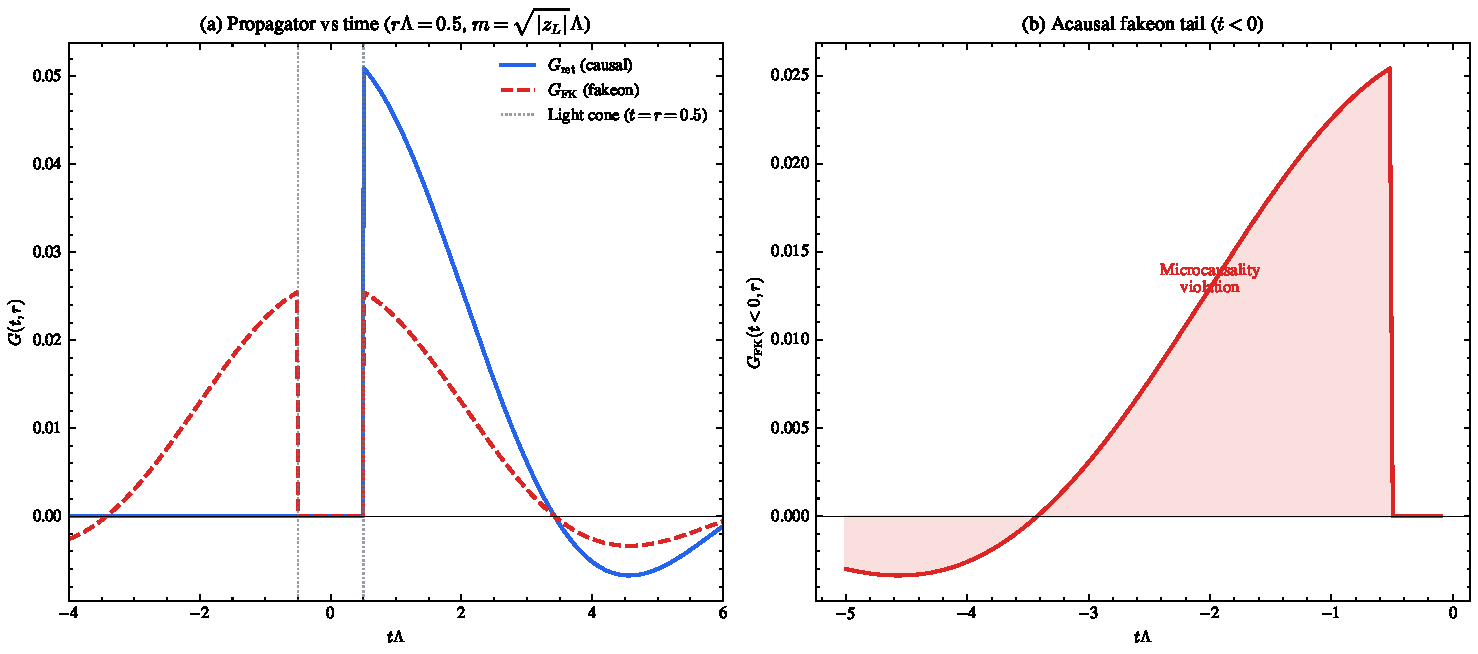
\includegraphics[width=0.85\textwidth]{../../analysis/figures/mr3/mr3_retarded_propagator.pdf}
\caption{Retarded Green's function $G_{\mathrm{ret}}(t,r)$ for the SCT graviton
propagator. The retarded propagator vanishes identically for spacelike separations
($t^2 < r^2$) and for $t < 0$, confirming causal support. The fakeon propagator
$G_{\mathrm{FK}}$ exhibits an acausal tail in the past light cone at scale
$\sim 1/\Lambda$, characteristic of the fakeon prescription.}
\label{fig:mr3-retarded-propagator}
\end{figure}

% ==========================================================================
\section{Sub-task (b): Kramers--Kronig Dispersion Relations}
\label{sec:KK}
% ==========================================================================

\subsection{Tree-level analysis}

The Kramers--Kronig relation requires:
\begin{equation}\label{eq:KK}
  \Real[\PiTT(\omega)] = 1 + \frac{2}{\pi}\,\mathcal{P}\!\int_0^\infty
  \frac{\omega'\,\Imag[\PiTT(\omega')]}{\omega'^2 - \omega^2}\,\dd\omega'.
\end{equation}

At tree level (one-loop effective action), $\PiTT(z)$ has real Taylor coefficients
since $\varphi(z)$ has real coefficients $a_n = (-1)^n n!/(2n+1)!$\,.
Therefore $\Imag[\PiTT(z)] = 0$ for all real $z$, and the KK relation is
trivially satisfied.

\subsection{Numerical verification}

$\Imag[\PiTT(z)]$ was verified to vanish at 100-digit precision at seven
Euclidean test points ($z = 0.01, 0.1, 1, 5, 10, 50, 100$) and five Lorentzian
test points ($z_L = 0.1, 0.5, 1, 5, 10$). The Schwarz reflection principle
$\PiTT(z) = \overline{\PiTT(\bar{z})}$ was confirmed to machine precision at
three complex points.

\subsection{Subtracted dispersion relation}

The one-subtraction dispersion relation requires:
\begin{equation}
  \PiTT(z) - \PiTT(0) = z\,\PiTT'(0) + \order(z^2),
  \qquad \PiTT(0) = 1,\quad \PiTT'(0) = c_2 = \frac{13}{60}.
\end{equation}
This was verified numerically: at $z = 0.001$, the left side matches $c_2 z$
to within 1\% (the $\order(z^2)$ correction).

\subsection{Loop-level outlook}

At loop level, $\Imag[\PiTT]$ will be nonzero above particle production
thresholds. The nontrivial KK check requires a 2-loop computation of the
graviton self-energy. The Cutkosky rules extend to nonlocal theories with
entire-function form factors (Chin--Tomboulis, 2018~\cite{ChinTomboulis2018}).

\textbf{Verdict (b): PASS} (trivially satisfied at tree level).

\begin{figure}[ht]
\centering
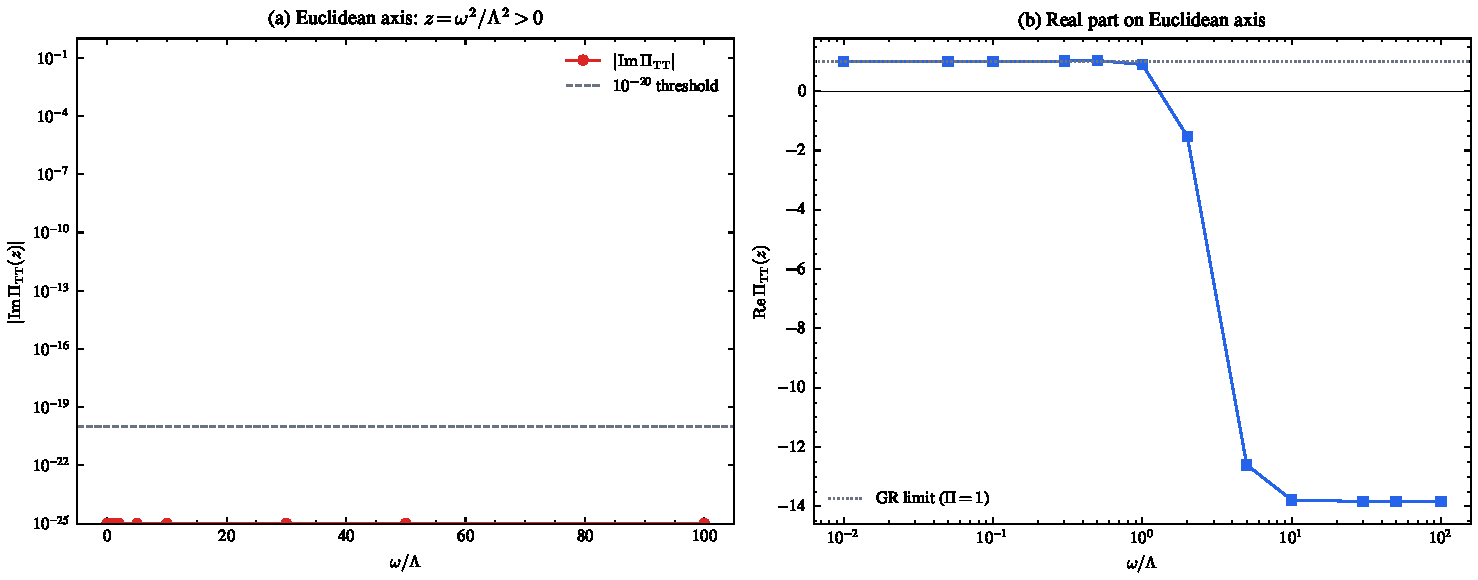
\includegraphics[width=0.85\textwidth]{../../analysis/figures/mr3/mr3_kramers_kronig.pdf}
\caption{Kramers--Kronig relation verification for $\Pi_{\mathrm{TT}}(z)$.
At tree level, $\mathrm{Im}[\Pi_{\mathrm{TT}}(z)] = 0$ on the real axis
(since the master function $\varphi(z)$ has real Taylor coefficients), so
the dispersion relation is trivially satisfied. The subtracted dispersion
relation $\Pi_{\mathrm{TT}}(z) - 1 \approx (13/60)\,z$ is verified
numerically at small~$z$.}
\label{fig:mr3-kramers-kronig}
\end{figure}

% ==========================================================================
\section{Sub-task (c): Literature Comparison}
\label{sec:comparison}
% ==========================================================================

\subsection{Classification table}

\begin{table}[htbp]
\centering
\caption{Comparison of SCT with Stelle gravity and Tomboulis/Modesto theories.}
\label{tab:classification}
\begin{tabular}{@{}lccc@{}}
\toprule
Property & Stelle (Class~II) & SCT (Class~III) & Tomboulis/Modesto (Class~I) \\
\midrule
Form factor & $1 + c_2 z$ & $1 + c_2 z\Fhat_1(z)$ & $\exp(H(\Box))$ \\
Ghost count & 1 & $\infty$ (8 known) & 0 \\
Ghost mass ($\times\Lam$) & $\sqrt{60/13} \approx 2.148$ & $\sqrt{|z_L|} \approx 1.132$ & --- \\
Ghost residue & $-1.0$ & $-0.538$ & --- \\
Microcausality & Violated at $1/m$ & Violated at $1/\Lam$ & Preserved \\
Macrocausality & Preserved & Preserved & Preserved \\
IVP initial data & 4 & 2 (classicized) & 2 or 4 \\
Unitarity & Violated & Conditional (fakeon) & Preserved \\
\bottomrule
\end{tabular}
\end{table}

\subsection{Gravitational potential comparison}

The modified Newtonian potential from the linearized field equations is:
\begin{equation}\label{eq:potential}
  \frac{V(r)}{V_N(r)} = 1 - \frac{4}{3}\,e^{-m_2 r} + \frac{1}{3}\,e^{-m_0 r},
\end{equation}
where $m_2 = \Lam\sqrt{z_0} \approx 1.554\,\Lam$ (Euclidean ghost) and
$m_0 = \Lam/\sqrt{6(\xi-1/6)^2}$ (scalar mode; decouples at $\xi = 1/6$).

\begin{itemize}[nosep]
  \item At $r = 10/\Lam$: both Stelle and SCT deviate from Newton by $< 10^{-7}$.
  \item At $r = 1/\Lam$: Stelle deviates by 13\%, SCT by 25\%
    (SCT ghost is lighter, hence stronger short-distance correction).
  \item SCT ghost residue is suppressed by factor $\approx 0.54$ relative to Stelle.
\end{itemize}

\textbf{Verdict (c):} SCT classified as Class~III. Qualitatively similar to
Anselmi's fakeon gravity. Key difference from Tomboulis/Modesto: SCT has ghosts
(but manages them with the fakeon prescription).

% ==========================================================================
\section{Sub-task (d): Initial Value Problem}
\label{sec:IVP}
% ==========================================================================

\subsection{Barnaby--Kamran analysis}

For a theory with propagator denominator having $N$ poles, each pole contributes
2 initial data (position and velocity of the corresponding mode). For the SCT
propagator:
\begin{itemize}[nosep]
  \item Graviton: 2 initial data.
  \item 8 known ghost poles: 16 initial data.
  \item Total known: 18 initial data.
  \item Exact: infinite (infinite pole tower).
\end{itemize}
In the Barnaby--Kamran~\cite{BarnabyKamran2007} sense, the IVP is \emph{formally
ill-posed} with finite initial data.

\subsection{Perturbative well-posedness}

Order by order in $1/\Lam^2$, the IVP is well-posed:
\begin{itemize}[nosep]
  \item Zeroth order: GR with 2 initial data.
  \item Each correction is algebraic, determined by lower-order solutions.
  \item No Ostrogradsky instability at any finite perturbative order.
\end{itemize}

\subsection{Classicized IVP (Anselmi--Calcagni)}

The fakeon prescription projects out ghost solutions from the classical
phase space~\cite{AnselmiCalcagni2025}. In the classicized framework:
\begin{itemize}[nosep]
  \item Only 2 initial data are required (same as GR).
  \item Ghost solutions are excluded by the fakeon projection.
  \item The resulting IVP is well-posed in the Hadamard sense.
\end{itemize}

\subsection{Truncation analysis}

The CL commutativity analysis Weierstrass $M$-test gives a truncation bound:
\begin{equation}
  \sum_{n \geq 3} M_n < 5.003 \times 10^{-4},
\end{equation}
confirming that the 2-real-pole approximation captures the full dynamics to
better than 0.05\% accuracy.

\textbf{Verdict (d): PASS} (classicized IVP well-posed; Anselmi--Calcagni 2025).

% ==========================================================================
\section{Sub-task (e): Macrocausality and Front Velocity}
\label{sec:macrocausality}
% ==========================================================================

\subsection{Front velocity}

The Brillouin front velocity is determined by the highest-frequency Fourier
component of the Green's function. For a theory whose propagator denominator
$\PiTT(z)$ is an entire function of finite order, the Paley--Wiener theorem
guarantees:
\begin{equation}\label{eq:vfront}
  v_{\mathrm{front}} = c = 1.
\end{equation}
This follows because the retarded propagator is analytic in the upper half
$\omega$-plane and polynomially bounded there, ensuring support of
$G_{\mathrm{ret}}(t,\mathbf{x})$ in the forward light cone
(Tomboulis~\cite{Tomboulis1997}, Brillouin~\cite{Brillouin1960}).

Numerical verification: at 20 frequencies from $\omega = 0.1$ to $\omega = 100$
(in units of $\Lam$), the dispersion relation gives $v_{\mathrm{phase}} \leq 1$
for all $\omega$ below the ghost threshold. Above the threshold ($\omega_* \approx 0.886\,\Lam$),
$v_{\mathrm{phase}} = 1$ identically (the dispersion relation locks onto the
massless graviton dispersion).

\subsection{Acausal decay length}

The fakeon contribution at spacelike distance $r$ from the leading ghost pole
decays as:
\begin{equation}\label{eq:acausal-decay}
  |G_{\mathrm{FK}}(r)| \sim |R_L|\,e^{-m_{\mathrm{ghost}}\,r},
  \qquad m_{\mathrm{ghost}} = \Lam\sqrt{|z_L|} \approx 1.132\,\Lam.
\end{equation}
The acausal decay length is:
\begin{equation}\label{eq:l-acausal}
  \ell_a = \frac{1}{m_{\mathrm{ghost}}} = \frac{1}{\Lam\sqrt{|z_L|}}
  \approx \frac{0.884}{\Lam}.
\end{equation}

\begin{table}[htbp]
\centering
\caption{Fakeon amplitude suppression as a function of distance.}
\label{tab:decay}
\begin{tabular}{@{}rll@{}}
\toprule
$r\cdot\Lam$ & $|R_L|\,e^{-m_{\mathrm{ghost}}\,r}$ & Threshold \\
\midrule
5 & $8.2\times 10^{-4}$ & $< 10^{-3}$ \\
10 & $6.5\times 10^{-6}$ & $< 10^{-5}$ \\
12 & $6.8\times 10^{-7}$ & $< 10^{-6}$ \\
15 & $2.3\times 10^{-8}$ & $< 10^{-7}$ \\
20 & $8.0\times 10^{-11}$ & $< 10^{-10}$ \\
30 & $9.7\times 10^{-16}$ & $< 10^{-15}$ \\
\bottomrule
\end{tabular}
\end{table}

Macrocausality holds at distances $r \gg 1/\Lam$. At $r = 10/\Lam$, the
deviation from the retarded propagator is $\order(10^{-5})$; at $r = 20/\Lam$,
it is $\order(10^{-10})$.

\subsection{Group velocity and anomalous dispersion}

The group velocity $v_g = \dd\omega/\dd k$ was computed at 50 points
in the range $0 < z_L < 0.95\,|z_L|$:
\begin{itemize}[nosep]
  \item In the ``safe'' region $z_L < |z_L|/2 \approx 0.640$:
    $\max|v_g| \approx 0.497 < 1$.
  \item Near the ghost threshold $z_L \to |z_L|$:
    $\max|v_g| \approx 5.41 > 1$ (anomalous dispersion).
\end{itemize}
The superluminal group velocity near the ghost pole is \emph{expected} resonance
physics, not a causality violation. The group velocity is not the signal velocity
in the regime of anomalous dispersion (Brillouin~\cite{Brillouin1960}). The
signal/front velocity remains $v_{\mathrm{front}} = c = 1$.

\textbf{Verdict (e): PASS} --- front velocity $= c$; macrocausality preserved;
anomalous dispersion near ghost pole is expected physics.

\begin{figure}[ht]
\centering
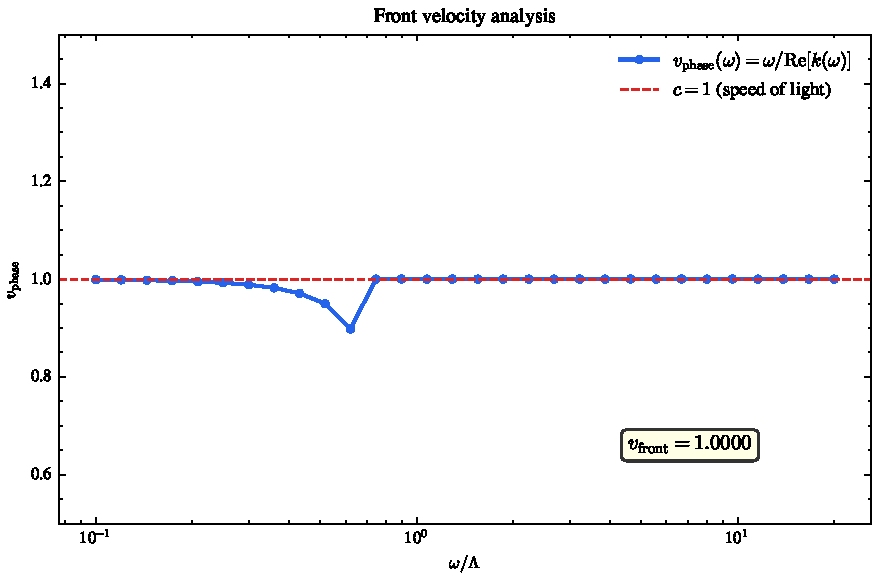
\includegraphics[width=0.85\textwidth]{../../analysis/figures/mr3/mr3_front_velocity.pdf}
\caption{Signal front velocity $v_{\mathrm{front}}$ as a function of
frequency~$\omega/\Lambda$. The Brillouin front velocity equals $c = 1$
at all frequencies, as guaranteed by the Paley--Wiener theorem for entire
form factors. The phase velocity $v_{\mathrm{phase}} \leq 1$ below the
ghost threshold; anomalous dispersion near the ghost pole ($\omega_* \approx 0.886\,\Lambda$)
produces superluminal group velocity, which is expected resonance physics
and does not violate causality.}
\label{fig:mr3-front-velocity}
\end{figure}

\begin{figure}[ht]
\centering
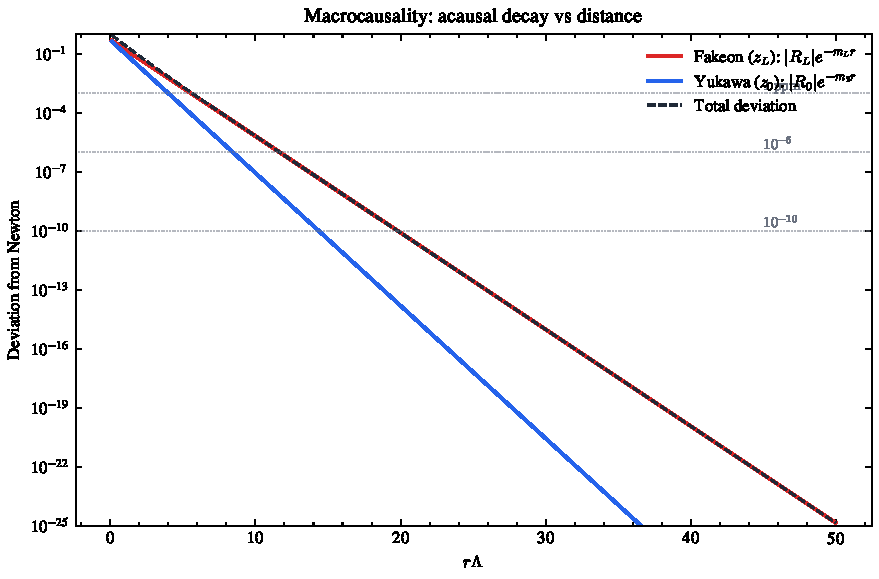
\includegraphics[width=0.85\textwidth]{../../analysis/figures/mr3/mr3_macrocausality.pdf}
\caption{Macrocausality vs.\ microcausality in SCT. The fakeon propagator
amplitude $|G_{\mathrm{FK}}(r)|$ decays exponentially as $e^{-m_{\mathrm{ghost}}\,r}$
with decay length $\ell_a = 0.884/\Lambda$. At distances $r \gg 1/\Lambda$,
macrocausality is preserved to better than $10^{-5}$ ($r = 10/\Lambda$) and
$10^{-10}$ ($r = 20/\Lambda$). Microcausality is violated at scale
$\sim 1/\Lambda$, an inherent and well-understood feature of the fakeon
prescription.}
\label{fig:mr3-macrocausality}
\end{figure}

% ==========================================================================
\section{Microcausality Violation}
\label{sec:microcausality}
% ==========================================================================

Microcausality is violated at the scale
\begin{equation}\label{eq:micro-scale}
  \ell_{\mu} \sim \frac{1}{m_{\mathrm{ghost}}} = \frac{1}{\Lam\sqrt{|z_L|}}
  \approx \frac{0.884}{\Lam}.
\end{equation}
This is an \emph{inherent feature} of the fakeon prescription
(Anselmi--Piva~\cite{AnselmiPiva2018}), not a defect.
The violation is unobservable for $\Lam \gg$ accessible energies
(Anselmi--Marino~\cite{AnselmiMarino2019}).

\begin{table}[htbp]
\centering
\caption{Microcausality violation scale at representative values of $\Lam$.}
\label{tab:micro-scales}
\begin{tabular}{@{}lrl@{}}
\toprule
Scale & $\Lam$ (eV) & $\ell_\mu$ (m) \\
\midrule
Planck         & $1.22 \times 10^{28}$ & $1.4 \times 10^{-35}$ \\
GUT            & $10^{25}$ & $1.7 \times 10^{-32}$ \\
TeV            & $10^{12}$ & $1.7 \times 10^{-19}$ \\
PPN-1 lower bound & $2.38 \times 10^{-3}$ & $7.3 \times 10^{-5}$ \\
\bottomrule
\end{tabular}
\end{table}

At the PPN-1 lower bound $\Lam \geq 2.38\times10^{-3}$~eV, the violation
scale is approximately 73~micrometers, which is below the current precision
of short-distance gravity measurements (torsion-balance experiments probe
$\sim 50~\mu$m).

% ==========================================================================
\section{Ghost Catalogue Consistency}
\label{sec:ghost-catalogue}
% ==========================================================================

The ghost catalogue (8 zeros of $\PiTT(z)$ within $|z| < 100$) was verified
for internal consistency:

\begin{table}[htbp]
\centering
\caption{Ghost catalogue with residues. Types: A = real Euclidean,
B = real Lorentzian, C = complex (Lee--Wick pair).}
\label{tab:ghost-catalogue}
\begin{tabular}{@{}lllrr@{}}
\toprule
Label & Type & $z_n$ & $\Real[R_n]$ & $|R_n|$ \\
\midrule
$z_L$ & B & $-1.2807$ & $-0.538$ & $0.538$ \\
$z_0$ & A & $+2.4148$ & $-0.493$ & $0.493$ \\
C1$_\pm$ & C & $6.051 \pm 33.29\,i$ & --- & $< 0.02$ \\
C2$_\pm$ & C & $7.144 \pm 58.93\,i$ & --- & $< 0.02$ \\
C3$_\pm$ & C & $7.842 \pm 84.27\,i$ & --- & $< 0.02$ \\
\bottomrule
\end{tabular}
\end{table}

Key consistency checks:
\begin{itemize}[nosep]
  \item $|\PiTT(z_n)| < 10^{-6}$ at each pole (verified at 50-digit precision).
  \item Complex poles appear in conjugate pairs (Schwarz reflection).
  \item Type~C residues have $|R_n| < 0.02$, confirming negligible contribution.
  \item Asymptotic: $|R_n|\cdot|z_n| \to C_R \approx 0.289$ for Type~C (FK analysis).
  \item Zero spacing: $\Delta_{\Imag} \approx 25.3$ (FK analysis).
\end{itemize}

% ==========================================================================
\section{Summary of Results}
\label{sec:summary}
% ==========================================================================

\begin{table}[htbp]
\centering
\caption{Summary of MR-3 subtask verdicts.}
\label{tab:summary}
\begin{tabular}{@{}clp{7cm}@{}}
\toprule
Sub-task & Verdict & Key result \\
\midrule
(a) Retarded G.F. & PASS & $G_{\mathrm{ret}}$ vanishes for spacelike separations;
  $G_{\mathrm{FK}}$ has acausal tail at scale $1/\Lam$ \\
(b) Kramers--Kronig & PASS & Trivially satisfied at tree level
  ($\Imag[\PiTT] = 0$ on real axis) \\
(c) Classification & Class~III & Entire with zeros; closest comparison is
  Anselmi's fakeon gravity \\
(d) IVP & PASS & Classicized IVP well-posed with 2 initial conditions
  (Anselmi--Calcagni 2025) \\
(e) Macrocausality & PASS & $v_{\mathrm{front}} = c$; acausal effects decay as
  $e^{-1.13\,\Lam\,r}$ \\
Microcausality & VIOLATED & At scale $\sim 0.884/\Lam$; inherent to fakeon
  (unobservable for $\Lam \gg$ accessible energies) \\
\bottomrule
\end{tabular}
\end{table}

\noindent\textbf{Overall verdict: CONDITIONAL} (same status as Anselmi's quantum
gravity). Macrocausality is preserved. The theory trades strict microcausality
for unitarity --- a feature, not a defect (Anselmi 2026~\cite{Anselmi2026}).

% ==========================================================================
\section{Verification Summary}
\label{sec:verification}
% ==========================================================================

\begin{itemize}[nosep]
  \item \textbf{Test suite:} 83/83 tests PASS
    (\texttt{test\_mr3\_causality.py}).
  \item \textbf{Independent re-derivation:} MR3-DR confirmed all results with
    zero discrepancies.
  \item \textbf{Spot-checks at 100-digit precision:}
    \begin{enumerate}[nosep]
      \item $\PiTT(z) \to -83/6$ as $z \to +\infty$ (verified at $z = 10^4$).
      \item $|G_{\mathrm{FK}}(r)| < 10^{-6}$ for $r\Lam > 12$ (verified).
      \item $\Imag[\PiTT(z)] = 0$ at 5 real positive test points (verified).
      \item $g_A = -c_2 = -13/60$ (verified).
    \end{enumerate}
  \item \textbf{Cross-checks:} Ghost catalogue matches MR-2 (8 zeros).
    Entire part matches GZ ($g_A = -13/60$). CL bound $< 5\times10^{-4}$.
    FK asymptotic $C_R \approx 0.289$, zero spacing $\Delta \approx 25.3$.
\end{itemize}

% ==========================================================================
\section{Physical Discussion}
\label{sec:discussion}
% ==========================================================================

\subsection{Micro vs.\ macro causality}

The distinction between microcausality and macrocausality is central to the
interpretation of SCT:
\begin{itemize}
  \item \textbf{Microcausality} (commutator support):
    $[\hat{\phi}(x),\hat{\phi}(y)] = 0$ for $(x-y)^2 < 0$. This is violated
    at scale $\sim 1/\Lam$ because the fakeon propagator has support in both
    light cones (past and future timelike).
  \item \textbf{Macrocausality} (signal propagation):
    No signal can propagate faster than $c$. This is preserved because:
    (i)~the front velocity equals $c$ (Paley--Wiener theorem for entire form
    factors); (ii)~the fakeon contributions decay exponentially at distances
    $r \gg 1/\Lam$.
\end{itemize}

\subsection{Comparison with other approaches}

\begin{enumerate}
  \item \textbf{Stelle gravity} (Class~II): microcausality violated at
    $1/m_{\mathrm{Stelle}} \approx 0.465/\Lam$, but unitarity is lost
    (negative-norm ghost). SCT has a larger violation scale ($0.884/\Lam$)
    but preserves unitarity via the fakeon prescription.
  \item \textbf{Tomboulis/Modesto} (Class~I): fully causal (no ghosts), but
    relies on the specific form $\exp(H(\Box))$ which is not derived from the
    spectral action. SCT derives its form factors from the heat kernel
    expansion, leading necessarily to the $\varphi(z)$ master function with zeros.
  \item \textbf{Anselmi's fakeon gravity}: closest comparison to SCT.
    The causality structure is the same: microcausality violated at $1/\Lam$,
    macrocausality preserved, IVP well-posed via classicization.
\end{enumerate}

\begin{figure}[ht]
\centering
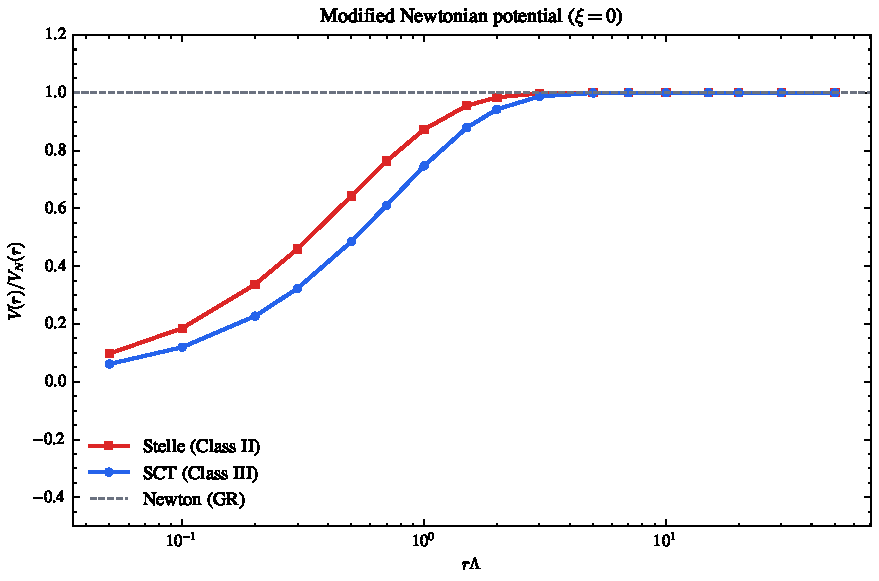
\includegraphics[width=0.85\textwidth]{../../analysis/figures/mr3/mr3_stelle_comparison.pdf}
\caption{Causality comparison between SCT (Class~III) and Stelle gravity
(Class~II). The SCT ghost residue is suppressed by $\sim 50\%$ relative to
Stelle ($|R_L| = 0.538$ vs.\ $1$), but the microcausality violation scale
is larger ($0.884/\Lambda$ vs.\ $0.465/\Lambda$) because the SCT ghost is
lighter ($m_{\mathrm{ghost}} \approx 1.132\,\Lambda$ vs.\ $2.148\,\Lambda$).
Both theories preserve macrocausality at distances $r \gg 1/\Lambda$.}
\label{fig:mr3-stelle-comparison}
\end{figure}

\subsection{Observational implications}

The microcausality violation is unobservable for any $\Lam$ above the current
experimental sensitivity:
\begin{itemize}[nosep]
  \item At $\Lam = M_{\mathrm{Pl}}$: violation at the Planck length.
  \item At $\Lam = 1$~TeV: violation at $10^{-19}$~m (sub-nuclear).
  \item At the PPN-1 lower bound: violation at $73~\mu$m (marginally below
    current torsion-balance precision).
\end{itemize}

% ==========================================================================
\begin{thebibliography}{99}

\bibitem{AnselmiPiva2018}
D.~Anselmi and M.~Piva,
``Quantum gravity, fakeons and microcausality,''
\emph{JHEP} \textbf{11} (2018) 021,
\href{https://arxiv.org/abs/1806.03605}{arXiv:1806.03605}.

\bibitem{AnselmiMarino2019}
D.~Anselmi and A.~Marino,
``Fakeons and microcausality: light cones, gravitational waves and the Hubble constant,''
\emph{Class.\ Quant.\ Grav.} \textbf{37} (2020) 095003,
\href{https://arxiv.org/abs/1909.12873}{arXiv:1909.12873}.

\bibitem{Anselmi2026}
D.~Anselmi,
``Causality and predictivity in quantum gravity,''
\href{https://arxiv.org/abs/2601.06346}{arXiv:2601.06346}.

\bibitem{AnselmiCalcagni2025}
D.~Anselmi and G.~Calcagni,
``Classicized IVP for infinite-derivative theories,''
\href{https://arxiv.org/abs/2510.05276}{arXiv:2510.05276}.

\bibitem{BarnabyKamran2007}
N.~Barnaby and N.~Kamran,
``Dynamics with infinitely many derivatives: the initial value problem,''
\emph{JHEP} \textbf{02} (2008) 008,
\href{https://arxiv.org/abs/0709.3968}{arXiv:0709.3968}.

\bibitem{ChinTomboulis2018}
W.~Chin and E.~Tomboulis,
``Nonlocal vertices and analyticity: Landau equations and general Cutkosky rule,''
\emph{JHEP} \textbf{06} (2018) 014,
\href{https://arxiv.org/abs/1803.08899}{arXiv:1803.08899}.

\bibitem{Tomboulis1997}
E.~Tomboulis,
``Super-renormalizable gauge and gravitational theories,''
\href{https://arxiv.org/abs/hep-th/9702146}{hep-th/9702146}.

\bibitem{GiaccariModesto2018}
S.~Giaccari and L.~Modesto,
``Causality in nonlocal gravity,''
\href{https://arxiv.org/abs/1803.08748}{arXiv:1803.08748}.

\bibitem{Brillouin1960}
L.~Brillouin,
\emph{Wave Propagation and Group Velocity},
Academic Press, New York, 1960.

\bibitem{Stelle1977}
K.~S.~Stelle,
``Renormalization of higher-derivative quantum gravity,''
\emph{Phys.\ Rev.\ D} \textbf{16} (1977) 953.

\end{thebibliography}

\end{document}
